\documentclass[10pt,aspectratio=43,mathserif,table]{beamer} 
%  设置为 Beamer 文档类型,设置字体为 10pt,长宽比为16:9,数学字体为 serif 风格
\batchmode
\usepackage{graphicx}
\usepackage{subfigure}
\usepackage{fontspec}

% \setmainfont{Harding Text Web Regular Regular.ttf}
\usepackage{diagbox} % 表头斜线分区
\usepackage{unicode-math}
\usefonttheme{serif}
% \setmathrm{Harding Text Web Regular Regular.ttf} % 设置数学字体为 Times New Roman
\setmathfont{TeX Gyre Termes Math} % 如果您使用 XeLaTeX 或 LuaLaTeX 编译,可以使用其他数学字体
\setmathtt{Courier New} % 设置等宽字体为 Courier New
\setboldmathrm{Times New Roman}
\setmathfont{TeX Gyre Termes Math}[version=bold] % 设置粗体数学字体
\setmathfont{TeX Gyre Termes Math}[range={\mathit}]


\usetheme{Berlin} %主题
\setbeamertemplate{page number in head/foot}[pagenumber]
%\usecolortheme{sustech} %主题颜色

\usepackage[ruled,linesnumbered]{algorithm2e}

\usepackage{fancybox}
\usepackage{xcolor}
\usepackage{listings}

\usepackage{booktabs}
\usepackage{colortbl}

\newcommand{\Console}{Console}
\lstset{ %
	backgroundcolor=\color{white},   % choose the background color
	basicstyle=\footnotesize\rmfamily,     % size of fonts used for the code
	columns=fullflexible,
	breaklines=true,                 % automatic line breaking only at whitespace
	captionpos=b,                    % sets the caption-position to bottom
	tabsize=4,
	commentstyle=\color{mygreen},    % comment style
	escapeinside={\%*}{*)},          % if you want to add LaTeX within your code
	keywordstyle=\color{blue},       % keyword style
	stringstyle=\color{mymauve}\ttfamily,     % string literal style
	numbers=left, 
	%	frame=single,
	rulesepcolor=\color{red!20!green!20!blue!20},
	% identifierstyle=\color{red},
	language=c
}


\definecolor{mygreen}{rgb}{0,0.6,0}
\definecolor{mymauve}{rgb}{0.58,0,0.82}
\definecolor{mygray}{gray}{.9}
\definecolor{mypink}{rgb}{.99,.91,.95}
\definecolor{mycyan}{cmyk}{.3,0,0,0}

%题目,作者,学校,日期
\title{Paper Reading}
%\subtitle{\fontsize{9pt}{14pt}\textbf{跨临界分岔}}
\author{Speaker: Yichen Lu\quad \newline  \newline \quad }
\institute{\fontsize{8pt}{14pt}}
\date{\today}
\newcommand{\concept}{Paper Reading}

%学校Logo
%\pgfdeclareimage[height=0.5cm]{sustech-logo}{sustech-logo.pdf}
%\logo{\pgfuseimage{sustech-logo}\hspace*{0.3cm}}

\AtBeginSection[]
{
	\begin{frame}<beamer>
	\frametitle{\textbf{Contents}}
	\tableofcontents[currentsection]
\end{frame}
}
% \beamerdefaultoverlayspecification{<+->}
% -----------------------------------------------------------------------------
\begin{document}
% -----------------------------------------------------------------------------
% \frame{\titlepage}
\begin{frame}
    \begin{figure}
        \centering
        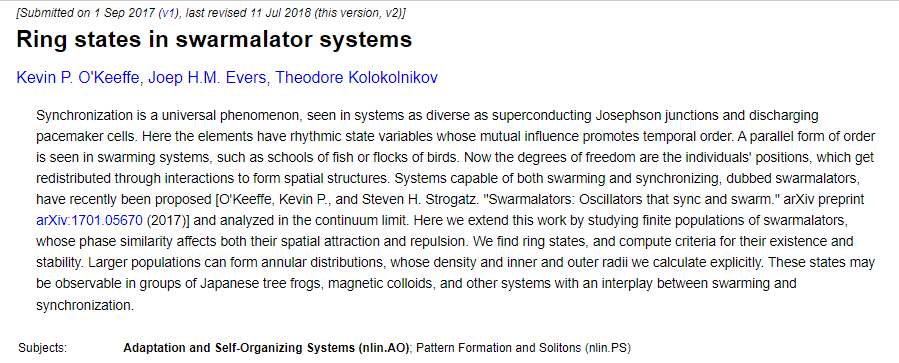
\includegraphics[width=\textwidth]{title.png}
    \end{figure}
\end{frame}

\begin{frame}
    Model equations:
    {
    \small
    $$
    \dot{\mathbf{x}}_k=\frac{1}{N}\sum_{j\ne i}^N{\left[ \left( \mathbf{x}_j-\mathbf{x}_k \right) \left( A+J_1\cos \left( \theta _j-\theta _k \right) \right) -\left( B-J_2\cos \left( \theta _j-\theta _k \right) \right) \frac{\mathbf{x}_j-\mathbf{x}_k}{\left| \mathbf{x}_j-\mathbf{x}_k \right|^2} \right]}
    $$
    $$
    \dot{\theta}_k=\frac{K}{N}\sum_{j\ne i}^N{\frac{\sin \left( \theta _j-\theta _k \right)}{\left| \mathbf{x}_j-\mathbf{x}_k \right|^2}}
    $$
    }
    $A=B=1$
\end{frame}

\begin{frame}{Ring phase waves}
    Spatial angle $\phi _k=\tan ^{-1}\left( \frac{\mathbf{x}_{k,2}}{\mathbf{x}_{k,1}} \right) $

    $ $

    In this state, the spatial angle of each swarmalator is correlated with its phase (i.e. $\phi _k=\theta _k + C$)

    $ $

    \textbf{Existence: } In the ring phase wave state, the position and phase of the $k$th swarmalator are

    $$
    \mathbf{x}_k=R\cos \left( 2\pi k/N \right) \hat{x}+R\sin \left( 2\pi k/N \right) \hat{y}
    $$
    $$
    \theta _k=2\pi k/N+C
    $$

    $$
    R=\sqrt{\frac{N-1+J_2}{N\left( 2-J_1 \right)}}
    $$

\end{frame}

\begin{frame}{Stability of Ring phase waves}
    When $K = 0$.
    $$
    J_{1a}:=\begin{cases}
        2-8\frac{\left( N-1+J_2 \right)}{\left( N-2 \right) ^2\left( 1-J_2 \right)},&		N\,\,even, N>4\\
        2-8\frac{\left( N-1+J_2 \right)}{\left( N-1 \right) \left( N-3 \right) \left( 1-J_2 \right)},&		N\,\,odd, N>4\\
    \end{cases}
    $$

    % In a classic paper [67], the stability of ring configurations of fluid vortices was studied, whose motion is controlled by the classic Helmholtz equations.

    When $K > 0$ the swarmalators’ phases are no longer frozen.
    
    $ $
    
    When $K < 0$
    $$
    J_{1b}:=\begin{cases}
        2\left( \frac{1}{1-4/N^2} \right) -\frac{1}{1-J_2}\frac{8}{\left( N-4/N \right)},&		N\,\,even, N>4\\
        2\left( \frac{1}{1-4/\left( N^2-1 \right)} \right) -\frac{1}{1-J_2}\frac{8}{\left( N-5/N \right)},&		N\,\,odd, N>4\\
    \end{cases}
    $$

    {
        \small
        $$
        K_{\mathrm{Hopf}}=\begin{cases}
            -\frac{\left( J_2-1 \right) \left( -2+J_1 \right) N^2+\left[ \left( -4J_2+4 \right) J_1+8J_2 \right] N+4J_1\left( J_2-1 \right)}{N\left( N-4 \right) \left( 2-J_1 \right)}\\
            -\frac{\left( J_2-1 \right) \left( -2+J_1 \right) N^2+\left[ \left( -4J_2+4 \right) J_1+8J_2 \right] N+\left( 3J_2-3 \right) J_1+2J_2-2}{\left( N^2-4N-1 \right) \left( 2-J_1 \right)}\\
        \end{cases}
        $$
    }
\end{frame}

\begin{frame}
    \begin{figure}
        \centering
        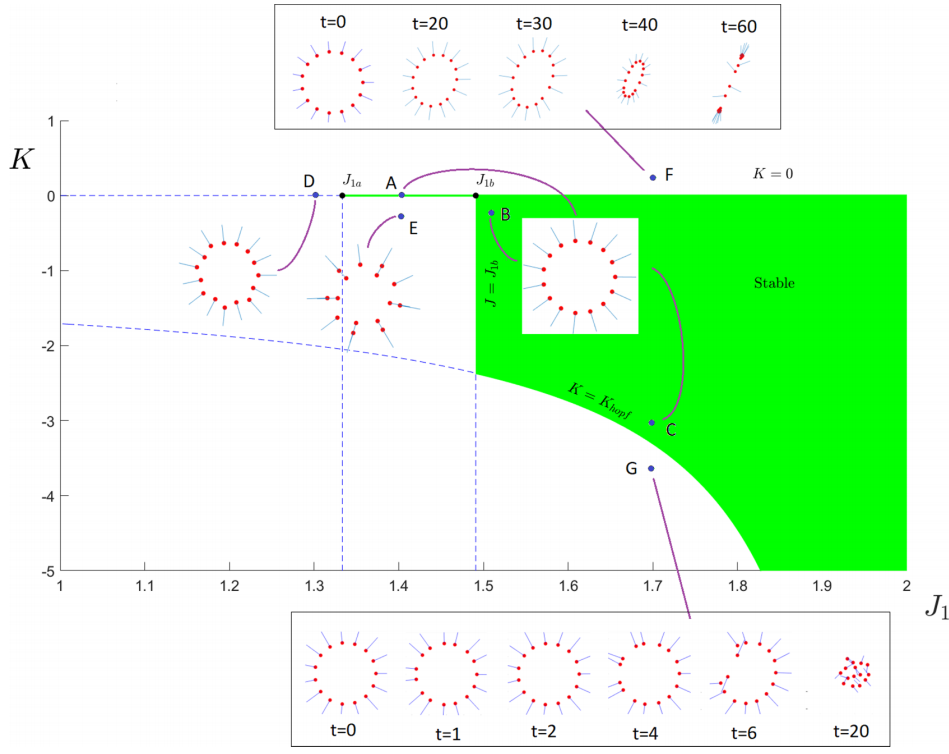
\includegraphics[width=0.8\textwidth]{f2.png}
    \end{figure}
\end{frame}

\begin{frame}
    $$
    N\rightarrow \infty , J_{1a}\sim J_{1b}\sim 2-\frac{8}{1-J_2}
    $$

    $$
    N_{\max}\sim \frac{8}{\left( 2-J_1 \right) \left( 1-J_2 \right)}
    $$


\end{frame}

\begin{frame}
    $$
    \begin{aligned}
        R_k&=\sqrt{\hat{x}_{k}^{2}+\hat{y}_{k}^{2}}\\
        S&=\sqrt{\frac{\sum\nolimits_{j=1}^N{\left( R_j-\bar{R} \right)}^2}{n-1}}\\
    \end{aligned}
    $$
\end{frame}

\begin{frame}
    
\end{frame}

\end{document}